% Created 2020-05-06 mié 14:02
% Intended LaTeX compiler: pdflatex
\documentclass[a4paper, 12pt]{article}
\usepackage[utf8]{inputenc}
\usepackage[T1]{fontenc}
\usepackage{graphicx}
\usepackage{grffile}
\usepackage{longtable}
\usepackage{wrapfig}
\usepackage{rotating}
\usepackage[normalem]{ulem}
\usepackage{amsmath}
\usepackage{textcomp}
\usepackage{amssymb}
\usepackage{capt-of}
\usepackage{hyperref}
\usepackage{float, amsfonts, commath, mathtools, proba}
\author{Tabaré Pérez}
\date{\today}
\title{Lecture 15 - 7: Prediction}
\hypersetup{
 pdfauthor={Tabaré Pérez},
 pdftitle={Lecture 15 - 7: Prediction},
 pdfkeywords={},
 pdfsubject={},
 pdfcreator={Emacs 26.3 (Org mode 9.3.6)}, 
 pdflang={English}}
\begin{document}

\maketitle
So now, we are ready to start looking at the question of prediction. So again,
as the same way as in the case of our discriminative supervised model, we will
have our points, let's say, just two classes, pluses and minuses.

\begin{figure}[H]
\centering
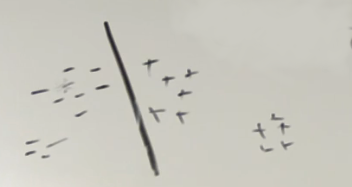
\includegraphics[width=0.5\textwidth]{./pic/u04-07-fig-01.png}
\caption{\label{fig:orgd4afa36}Discriminative supervised model}
\end{figure}

And using the estimation techniques, as I just described to you earlier, we can
actually induce the probability distribution: find \(\theta\)s.

Find \(\theta\)s for plus points, \(\theta^+\), and also, find \(\theta\)s for
minus points, \(\theta^-\).

Find the parameters for thes classes in such a way that they will give the
highest likelihood to the points, for instance, on the plus side.

So now, the question is, if I give you a new document, how do you know to which
class it belongs?

So one way to think about it is to say, I have my document and I could look
at the likelihood that this document was generated by plus side:

\begin{equation}
\prob(D|\theta^+)
\end{equation}

Also I could look at the likelihood that this document is generated by the minus
class:

\begin{equation}
\prob(D|\theta^-)
\end{equation}

And look its log:

\begin{equation}
\log \left( \frac{\prob(D|\theta^{+})}{\prob(D|\theta^{-})} \right)
\end{equation}

You can ask me why I am looking at the log. You will see later.

But the point is, intuitively speaking, we would want to see that the document
will be assigned to the class which gives to it the higher likelihood. And for
now, I will make one assumption, which I am going to break later. Let's make an
assumption that the likelihood of a document in the minus class (the prior
likelihood of the minus class) and in the plus class are exactly the same.

So in this particular case, we are going to be looking at this log:

\begin{equation}
\log \left( \frac{\prob(D|\theta^{+})}{\prob(D|\theta^{-})} \right) \left\{ \begin{array}{ll}
                                                                            +, & if \geq 0\\
                                                                            -, & otherwise
                                                                            \end{array}
                                                                    \right.                                                                      
\end{equation}


And we would say that if it is bigger or equal to zero, then we are going to
return plus. and if it is smaller than zero, we are going to return the minus.

So these type of distributions are called \textbf{class conditional distributions} so
that you just know.

So let's just look more closely. I am going to just open up this expression and
massage it in a different way. And eventually, I will bring it to you to the
form that you've already seen in the past. But let's just start. So again, we
have here log of this ratio and we can just write it as log of one expression
minus the log of another expression:

\begin{equation}
\log \prob(D|\theta^+) - \log \prob(D|\theta^-) = \log \prod_{w \in \mathcal{W}} \theta^{+^{\text{count}(w)}} - \log \prod_{w \in \mathcal{W}} \theta^{-^{\text{count}(w)}} =
\end{equation}

So now, we can continue to do some manipulation. and again, we'll remember that
log of the product is the sum of logs:

\begin{equation}
= \sum_{w \in \mathcal{W}} \text{count}(w) \cdot \log(\theta_{w}^{+}) - \sum_{w \in \mathcal{W}} \text{count}(w) \cdot \log(\theta_{w}^{-}) =
\end{equation}

So I will do my almost last rearrangement here:

\begin{equation}
= \sum_{w \in \mathcal{W}} \text{count}(w) \cdot \overbrace{\log \left(\frac{\theta_{w}^{+}}{\theta_{w}^{-}}\right)}^{\hat{\theta}_{w}} =
\end{equation}

And the last thing that I'm going to do, this is truly the last thing, I am
going to just use to introduce for you and a new notation.

So instead of writing this big expression, , I'm going to just call it like
\(\hat{\theta}_w\). So I'm just writing it here:

\begin{equation}
= \sum_{w \in \mathcal{W}} \text{count}(w) \cdot \hat{\theta}_w
\end{equation}

And you would immediately see why it is a good idea.

So if you are now looking at this,  so remember we started here:

\begin{equation}
\log \left( \frac{\prob(D|\theta^{+})}{\prob(D|\theta^{-})} \right) = \sum_{w \in \mathcal{W}} \text{count}(w) \cdot \hat{\theta}_w
\end{equation}

So at this point, looking at this expression, which we derived looking through
generative view on classification, actually what we got here should remind you a
linear classifier that goes through origin with respect to this parameter
\(\hat{\theta}_w\) . So despite the fact that we went kind of in a very
different way, what we got with our generative model, is a linear
classifier, just get there in a different way.
\end{document}